% Options for packages loaded elsewhere
\PassOptionsToPackage{unicode}{hyperref}
\PassOptionsToPackage{hyphens}{url}
%
\documentclass[
  a4paper,
]{article}
\usepackage{amsmath,amssymb}
\usepackage{iftex}
\ifPDFTeX
  \usepackage[T1]{fontenc}
  \usepackage[utf8]{inputenc}
  \usepackage{textcomp} % provide euro and other symbols
\else % if luatex or xetex
  \usepackage{unicode-math} % this also loads fontspec
  \defaultfontfeatures{Scale=MatchLowercase}
  \defaultfontfeatures[\rmfamily]{Ligatures=TeX,Scale=1}
\fi
\usepackage{lmodern}
\ifPDFTeX\else
  % xetex/luatex font selection
  \setmainfont[]{Helvetica}
\fi
% Use upquote if available, for straight quotes in verbatim environments
\IfFileExists{upquote.sty}{\usepackage{upquote}}{}
\IfFileExists{microtype.sty}{% use microtype if available
  \usepackage[]{microtype}
  \UseMicrotypeSet[protrusion]{basicmath} % disable protrusion for tt fonts
}{}
\makeatletter
\@ifundefined{KOMAClassName}{% if non-KOMA class
  \IfFileExists{parskip.sty}{%
    \usepackage{parskip}
  }{% else
    \setlength{\parindent}{0pt}
    \setlength{\parskip}{6pt plus 2pt minus 1pt}}
}{% if KOMA class
  \KOMAoptions{parskip=half}}
\makeatother
\usepackage{xcolor}
\usepackage[margin=1in]{geometry}
\usepackage{graphicx}
\makeatletter
\def\maxwidth{\ifdim\Gin@nat@width>\linewidth\linewidth\else\Gin@nat@width\fi}
\def\maxheight{\ifdim\Gin@nat@height>\textheight\textheight\else\Gin@nat@height\fi}
\makeatother
% Scale images if necessary, so that they will not overflow the page
% margins by default, and it is still possible to overwrite the defaults
% using explicit options in \includegraphics[width, height, ...]{}
\setkeys{Gin}{width=\maxwidth,height=\maxheight,keepaspectratio}
% Set default figure placement to htbp
\makeatletter
\def\fps@figure{htbp}
\makeatother
\setlength{\emergencystretch}{3em} % prevent overfull lines
\providecommand{\tightlist}{%
  \setlength{\itemsep}{0pt}\setlength{\parskip}{0pt}}
\setcounter{secnumdepth}{-\maxdimen} % remove section numbering
\usepackage{titling}
\pretitle{\begin{flushleft}}
\posttitle{\end{flushleft}}
\usepackage{booktabs}
\usepackage{longtable}
\usepackage{float}
\usepackage{colortbl}
\usepackage{pdflscape}
\usepackage{tabu}
\usepackage{makecell}
\usepackage{xcolor}
\usepackage{soul}
\usepackage{caption}
\usepackage[singlelinecheck=false]{caption}
\usepackage[font={footnotesize,it}]{caption}
\usepackage{booktabs}
\usepackage{longtable}
\usepackage{array}
\usepackage{multirow}
\usepackage{wrapfig}
\usepackage{float}
\usepackage{colortbl}
\usepackage{pdflscape}
\usepackage{tabu}
\usepackage{threeparttable}
\usepackage{threeparttablex}
\usepackage[normalem]{ulem}
\usepackage{makecell}
\usepackage{xcolor}
\ifLuaTeX
  \usepackage{selnolig}  % disable illegal ligatures
\fi
\usepackage{bookmark}
\IfFileExists{xurl.sty}{\usepackage{xurl}}{} % add URL line breaks if available
\urlstyle{same}
\hypersetup{
  hidelinks,
  pdfcreator={LaTeX via pandoc}}

\title{\vspace{-1.5cm} \begin{LARGE} WGS Quality Control Report \end{LARGE}}
\author{}
\date{\vspace{-2.5em}}

\begin{document}
\maketitle

\normalsize Batch Name: 2024-07-04

\normalsize Experiment Name: 24ARS\_EMR\_LG788

\fontsize{7}{8}
\selectfont
\captionsetup[table]{labelformat=empty}
\renewcommand{\arraystretch}{1.2}

\begin{longtable}[t]{>{\centering\arraybackslash}p{1cm}>{\centering\arraybackslash}p{2cm}>{\centering\arraybackslash}p{1.5cm}>{\centering\arraybackslash}p{5.25cm}>{\centering\arraybackslash}p{5.25cm}}
\toprule
\multicolumn{1}{>{\centering\arraybackslash}p{1cm}}{\cellcolor[HTML]{D4D4D4}{\textbf{Isolate No.}}} & \multicolumn{1}{>{\centering\arraybackslash}p{2cm}}{\cellcolor[HTML]{D4D4D4}{\textbf{Sample ID}}} & \multicolumn{1}{>{\centering\arraybackslash}p{1.5cm}}{\cellcolor[HTML]{D4D4D4}{\textbf{Description}}} & \multicolumn{1}{>{\centering\arraybackslash}p{5.25cm}}{\cellcolor[HTML]{D4D4D4}{\textbf{ARSRL}}} & \multicolumn{1}{>{\centering\arraybackslash}p{5.25cm}}{\cellcolor[HTML]{D4D4D4}{\textbf{WGS}}}\\
\midrule
1 & 23ARS\_VSM0511 & SAL68 & Salmonella species & \cellcolor{white}{Salmonella enterica subsp. enterica serovar Enteritidis}\\
2 & 24ARS\_BRH0014 & EMR142\_2 & Pseudomonas aeruginosa & \cellcolor{white}{Pseudomonas aeruginosa}\\
3 & 24ARS\_BRT0017 & EMR141\_2 & Pseudomonas aeruginosa & \cellcolor{white}{Pseudomonas aeruginosa}\\
4 & 24ARS\_CRH0017 & EMR146 & Escherichia coli & \cellcolor{white}{Escherichia coli}\\
5 & 24ARS\_CRH0030 & EMR148 & Klebsiella pneumoniae & \cellcolor{white}{Klebsiella quasipneumoniae}\\
\addlinespace
6 & 24ARS\_DMC0098 & EMR149 & Klebsiella pneumoniae & \cellcolor{white}{Klebsiella pneumoniae}\\
7 & 24ARS\_DMC0102 & EMR157 & Pseudomonas aeruginosa & \cellcolor{white}{Pseudomonas aeruginosa}\\
8 & 24ARS\_EVR0011 & EMR155 & Pseudomonas aeruginosa & \cellcolor{white}{Pseudomonas aeruginosa}\\
9 & 24ARS\_EVR0017 & EMR158 & Pseudomonas aeruginosa & \cellcolor{white}{Pseudomonas aeruginosa}\\
10 & 24ARS\_GMH0029 & EMR145 & Klebsiella pneumoniae & \cellcolor{white}{Klebsiella pneumoniae}\\
\addlinespace
11 & 24ARS\_JLM0018 & EMR143 & Klebsiella pneumoniae & \cellcolor{white}{Klebsiella pneumoniae}\\
12 & 24ARS\_JLM0020 & EMR144 & Klebsiella pneumoniae & \cellcolor{white}{Klebsiella quasipneumoniae}\\
13 & 24ARS\_NKI0048 & EMR147 & Escherichia coli & \cellcolor{white}{Escherichia coli}\\
14 & 24ARS\_NKI0050 & EMR150 & Klebsiella pneumoniae & \cellcolor{white}{Klebsiella pneumoniae}\\
15 & 24ARS\_NKI0051 & EMR151 & Klebsiella pneumoniae & \cellcolor{white}{Klebsiella pneumoniae}\\
\addlinespace
16 & 24ARS\_SLH0030 & EMR154 & Pseudomonas aeruginosa & \cellcolor{white}{Pseudomonas aeruginosa}\\
17 & 24ARS\_STU0024 & EMR152 & Klebsiella pneumoniae & \cellcolor{white}{Klebsiella pneumoniae}\\
18 & 24ARS\_STU0027 & EMR153 & Acinetobacter baumannii & \cellcolor{white}{Acinetobacter pittii}\\
\cellcolor[HTML]{FFA77F}{19} & \cellcolor[HTML]{FFA77F}{24ARS\_ZMC0002} & \cellcolor[HTML]{FFA77F}{EMR156} & \cellcolor[HTML]{FFA77F}{Pseudomonas aeruginosa} & \cellcolor[HTML]{FFA77F}{Pseudomonas aeruginosa}\\
20 & UTP\_BL\_006 & tricycle & Escherichia coli & \cellcolor{white}{Escherichia coli}\\
\addlinespace
21 & UTP\_ST\_031 & tricycle & Escherichia coli & \cellcolor{white}{Escherichia coli}\\
\bottomrule
\end{longtable}

\tiny Legend: \begingroup\fontsize{4}{6}\selectfont

\begin{tabular}{|>{\centering\arraybackslash}p{1cm}|>{\centering\arraybackslash}p{1cm}|>{\centering\arraybackslash}p{1cm}|>{\centering\arraybackslash}p{3cm}|>{\centering\arraybackslash}p{2cm}|}

\cellcolor{white}{PASS} & \cellcolor[HTML]{FFA77F}{WARNING} & \cellcolor[HTML]{FD7979}{FAILURE} & \textcolor{blue}{EXCEEDS THRESHOLD METRIC/S} & \cellcolor{yellow}{NON-CONCORDANT}\\

\end{tabular}
\endgroup{}
\fontsize{7}{8}
\selectfont
\captionsetup[table]{labelformat=empty}
\renewcommand{\arraystretch}{1.2}

\begin{tabular}{>{\centering\arraybackslash}p{3cm}>{\centering\arraybackslash}p{3cm}>{\centering\arraybackslash}p{2cm}>{\centering\arraybackslash}p{7cm}}
\toprule
\multicolumn{4}{l}{\textbf{Sample excluded in the analysis}} \\
\cmidrule(l{3pt}r{3pt}){1-4}
\multicolumn{1}{>{\centering\arraybackslash}p{3cm}}{\cellcolor[HTML]{D4D4D4}{\textbf{Sample ID}}} & \multicolumn{1}{>{\centering\arraybackslash}p{3cm}}{\cellcolor[HTML]{D4D4D4}{\textbf{Description}}} & \multicolumn{1}{>{\centering\arraybackslash}p{2cm}}{\cellcolor[HTML]{D4D4D4}{\textbf{Index reads}}} & \multicolumn{1}{>{\centering\arraybackslash}p{7cm}}{\cellcolor[HTML]{D4D4D4}{\textbf{Remarks}}}\\
\midrule
24ARS\_NKI0053 & EMR159 & 0.8429 & low read count\\
\bottomrule
\end{tabular}

\(\\\)

\fontsize{7}{8}
\selectfont
\captionsetup[table]{labelformat=empty}
\renewcommand{\arraystretch}{1.2}

\begin{longtable}[t]{>{\centering\arraybackslash}p{1cm}>{\centering\arraybackslash}p{3cm}>{\centering\arraybackslash}p{2cm}>{\centering\arraybackslash}p{2cm}>{\centering\arraybackslash}p{2cm}>{\centering\arraybackslash}p{2cm}>{\centering\arraybackslash}p{2cm}}
\toprule
\multicolumn{1}{>{\centering\arraybackslash}p{1cm}}{\cellcolor[HTML]{D4D4D4}{\textbf{Isolate No.}}} & \multicolumn{1}{>{\centering\arraybackslash}p{3cm}}{\cellcolor[HTML]{D4D4D4}{\textbf{Sample ID}}} & \multicolumn{1}{>{\centering\arraybackslash}p{2cm}}{\cellcolor[HTML]{D4D4D4}{\textbf{Contamination}}} & \multicolumn{1}{>{\centering\arraybackslash}p{2cm}}{\cellcolor[HTML]{D4D4D4}{\textbf{Contigs}}} & \multicolumn{1}{>{\centering\arraybackslash}p{2cm}}{\cellcolor[HTML]{D4D4D4}{\textbf{GC Percent}}} & \multicolumn{1}{>{\centering\arraybackslash}p{2cm}}{\cellcolor[HTML]{D4D4D4}{\textbf{N50}}} & \multicolumn{1}{>{\centering\arraybackslash}p{2cm}}{\cellcolor[HTML]{D4D4D4}{\textbf{Total Length}}}\\
\midrule
1 & 23ARS\_VSM0511 & \textcolor{black}{0} & \textcolor{black}{24} & 52.13 & \textcolor{black}{478941} & 4700439\\
2 & 24ARS\_BRH0014 & \textcolor{black}{0} & \textcolor{black}{84} & 65.97 & \textcolor{black}{247991} & 6878546\\
3 & 24ARS\_BRT0017 & \textcolor{black}{0} & \textcolor{black}{122} & 65.33 & \textcolor{black}{220628} & 7348540\\
4 & 24ARS\_CRH0017 & \textcolor{black}{0} & \textcolor{black}{127} & 50.53 & \textcolor{black}{136602} & 5373741\\
5 & 24ARS\_CRH0030 & \textcolor{black}{0} & \textcolor{black}{39} & 57.75 & \textcolor{black}{801312} & 5379490\\
\addlinespace
6 & 24ARS\_DMC0098 & \textcolor{black}{0} & \textcolor{black}{44} & 57.19 & \textcolor{black}{479099} & 5405179\\
7 & 24ARS\_DMC0102 & \textcolor{black}{0} & \textcolor{black}{51} & 66.32 & \textcolor{black}{488628} & 6482852\\
8 & 24ARS\_EVR0011 & \textcolor{black}{0} & \textcolor{black}{47} & 66.47 & \textcolor{black}{407140} & 6291421\\
9 & 24ARS\_EVR0017 & \textcolor{black}{0} & \textcolor{black}{131} & 66.36 & \textcolor{black}{151006} & 6423637\\
10 & 24ARS\_GMH0029 & \textcolor{black}{0} & \textcolor{black}{110} & 56.65 & \textcolor{black}{172819} & 5772594\\
\addlinespace
11 & 24ARS\_JLM0018 & \textcolor{black}{0} & \textcolor{black}{95} & 56.79 & \textcolor{black}{394359} & 5742923\\
12 & 24ARS\_JLM0020 & \textcolor{black}{0} & \textcolor{black}{77} & 57.65 & \textcolor{black}{229344} & 5512178\\
13 & 24ARS\_NKI0048 & \textcolor{black}{0} & \textcolor{black}{93} & 50.83 & \textcolor{black}{320376} & 5148168\\
14 & 24ARS\_NKI0050 & \textcolor{black}{0} & \textcolor{black}{55} & 57.20 & \textcolor{black}{236088} & 5425644\\
15 & 24ARS\_NKI0051 & \textcolor{black}{0} & \textcolor{black}{81} & 56.82 & \textcolor{black}{238924} & 5595191\\
\addlinespace
16 & 24ARS\_SLH0030 & \textcolor{black}{0} & \textcolor{black}{99} & 65.94 & \textcolor{black}{361062} & 6937344\\
17 & 24ARS\_STU0024 & \textcolor{black}{0} & \textcolor{black}{55} & 57.13 & \textcolor{black}{303929} & 5493891\\
18 & 24ARS\_STU0027 & \textcolor{black}{0} & \textcolor{black}{17} & 38.58 & \textcolor{black}{519454} & 3995354\\
\cellcolor[HTML]{FFA77F}{19} & \cellcolor[HTML]{FFA77F}{24ARS\_ZMC0002} & \cellcolor[HTML]{FFA77F}{\textcolor{black}{0}} & \cellcolor[HTML]{FFA77F}{\textcolor{black}{89}} & \cellcolor[HTML]{FFA77F}{66.46} & \cellcolor[HTML]{FFA77F}{\textcolor{black}{197528}} & \cellcolor[HTML]{FFA77F}{6319285}\\
20 & UTP\_BL\_006 & \textcolor{black}{0} & \textcolor{black}{44} & 50.61 & \textcolor{black}{279880} & 4940847\\
\addlinespace
21 & UTP\_ST\_031 & \textcolor{black}{0} & \textcolor{black}{109} & 50.42 & \textcolor{black}{166206} & 5380880\\
\bottomrule
\end{longtable}

\tiny Legend: \begingroup\fontsize{4}{6}\selectfont

\begin{tabular}{|>{\centering\arraybackslash}p{1cm}|>{\centering\arraybackslash}p{1cm}|>{\centering\arraybackslash}p{1cm}|>{\centering\arraybackslash}p{2.5cm}|>{\centering\arraybackslash}p{8cm}|}

\cellcolor{white}{PASS} & \cellcolor[HTML]{FFA77F}{WARNING} & \cellcolor[HTML]{FD7979}{FAILURE} & \textcolor{blue}{EXCEEDS THRESHOLD METRIC/S} & *Isolates were tagged with warning due to uncertain results  of species identification using bactinspector or sequence identification levels.\\

\end{tabular}
\endgroup{}

\fontsize{7}{8}
\selectfont
\captionsetup[table]{labelformat=empty}
\renewcommand{\arraystretch}{1.2}

\begin{longtable}[l]{>{\centering\arraybackslash}p{3cm}>{\centering\arraybackslash}p{12cm}}
\toprule
\multicolumn{2}{l}{\textbf{List of samples above/below QC threshold metrics}} \\
\cmidrule(l{3pt}r{3pt}){1-2}
\cellcolor[HTML]{D4D4D4}{\textbf{Sample ID}} & \cellcolor[HTML]{D4D4D4}{\textbf{Remarks}}\\
\midrule
 & No QC failures found.\\
\bottomrule
\end{longtable}

\fontsize{7}{8}
\selectfont
\captionsetup[table]{labelformat=empty}
\renewcommand{\arraystretch}{1.2}

\begin{longtable}[l]{>{\raggedright\arraybackslash}p{8cm}c}
\toprule
\cellcolor[HTML]{D4D4D4}{\textbf{WGS\_ID}} & \cellcolor[HTML]{D4D4D4}{\textbf{Number}}\\
\midrule
Pseudomonas aeruginosa & 7\\
Klebsiella pneumoniae & 6\\
Escherichia coli & 4\\
Klebsiella quasipneumoniae & 2\\
Acinetobacter pittii & 1\\
\addlinespace
Salmonella enterica subsp. enterica serovar Enteritidis & 1\\
\bottomrule
\end{longtable}

\begin{itemize}
\item
  \(\color{red}6\) distinct species were identified among
  \(\color{red}21\) isolates.
\item
  \(\color{red}95.24\) \% (n=20) of the isolates passed the QC, while
  \(\color{red}4.76\) \% (n=1) were tagged with warning.
\item
  Concordance between ARSRL and WGS species report was
  \(\color{red}100.00\) \%. \(\\\)
\end{itemize}

\subsubsection{GRAPHS}\label{graphs}

\fontsize{7}{8}
\selectfont
\captionsetup[table]{labelformat=empty}
\renewcommand{\arraystretch}{1.2}

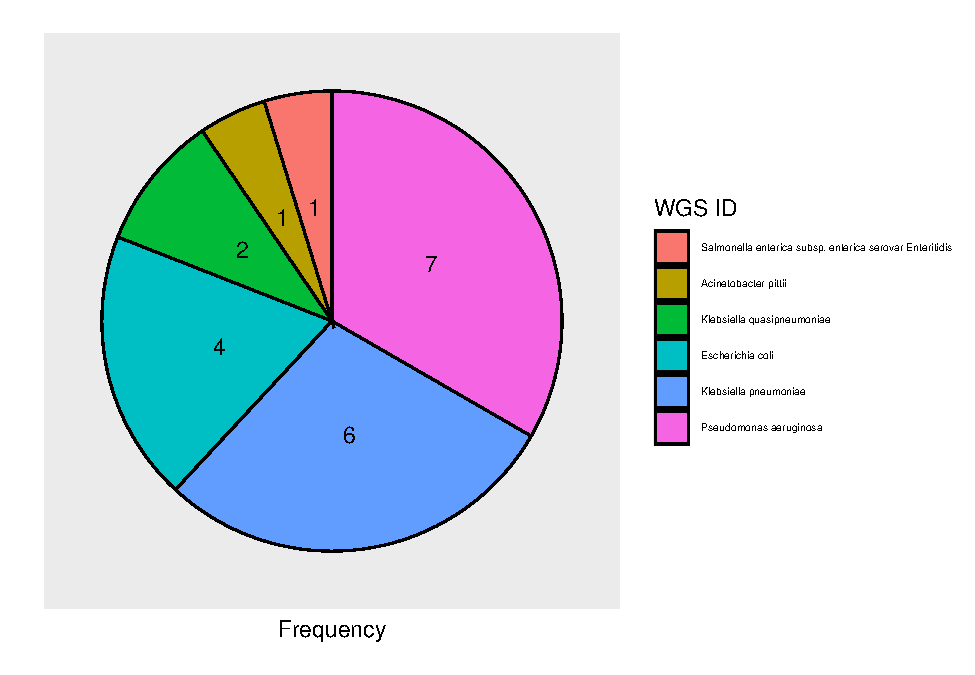
\includegraphics{qualifyr_report_2024-07-04_files/figure-latex/pie_chart-1.pdf}

\subsubsection{Result Classification}\label{result-classification}

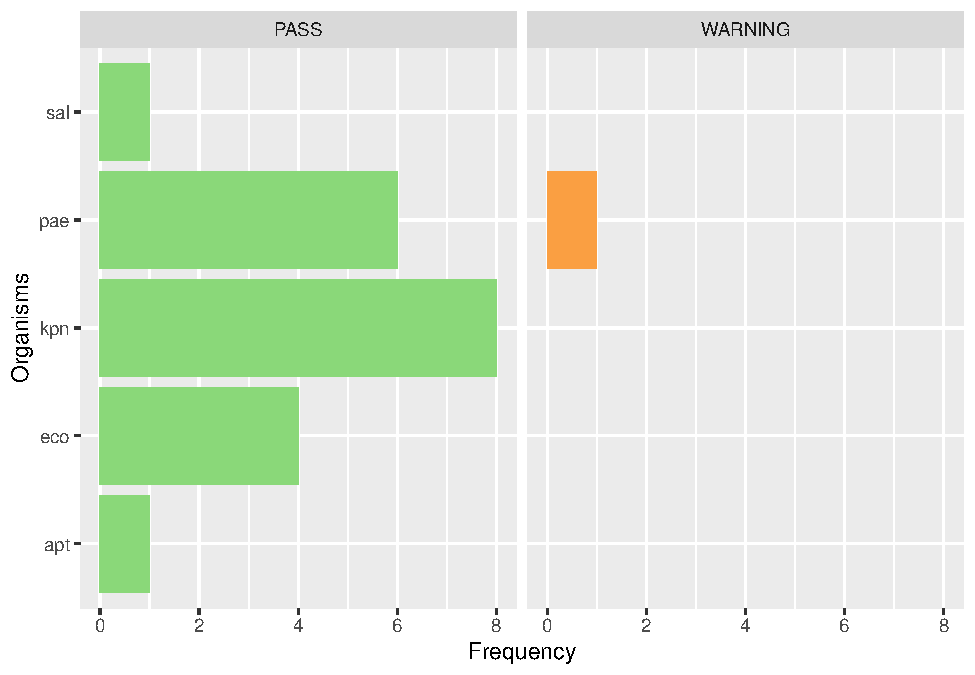
\includegraphics{qualifyr_report_2024-07-04_files/figure-latex/organism results-1.pdf}

\subsubsection{Number of contigs}\label{number-of-contigs}

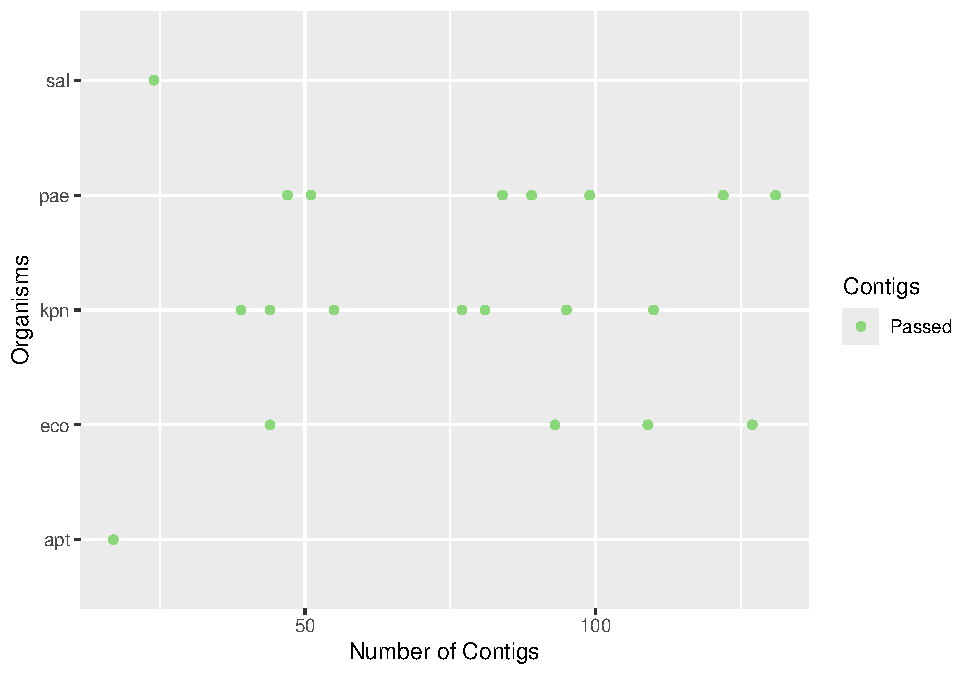
\includegraphics{qualifyr_report_2024-07-04_files/figure-latex/unnamed-chunk-1-1.pdf}

\subsubsection{N50 Value}\label{n50-value}

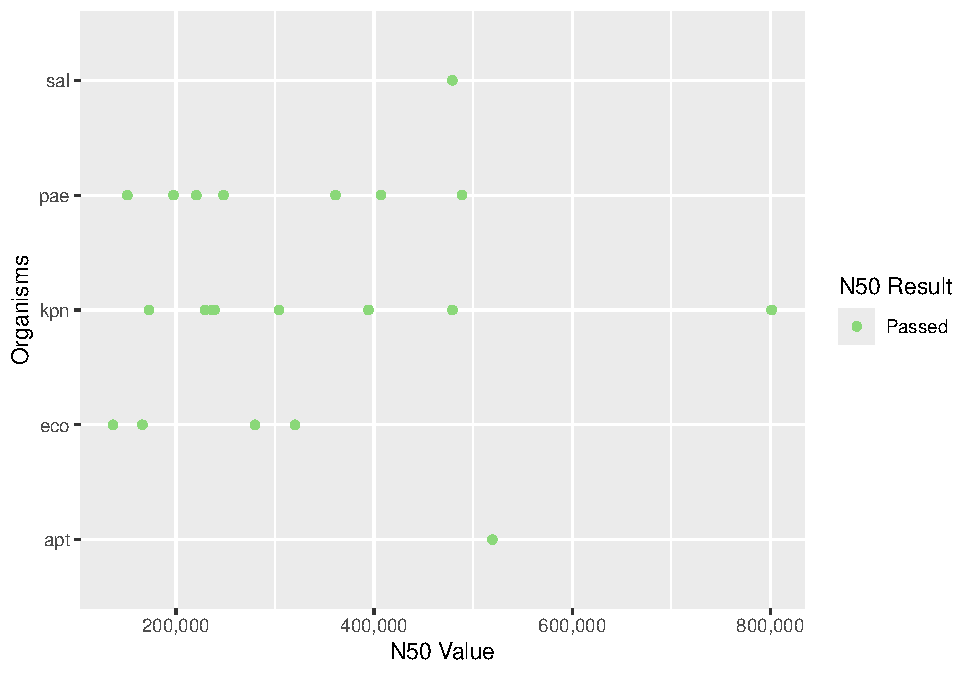
\includegraphics{qualifyr_report_2024-07-04_files/figure-latex/n50_result -1.pdf}

\subsubsection{Total Length}\label{total-length}

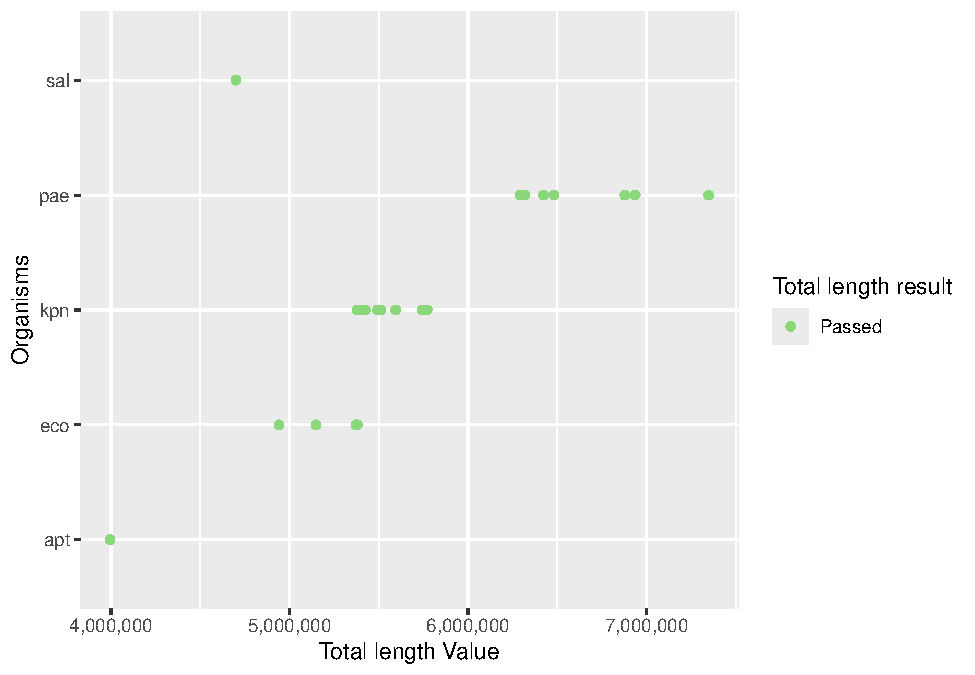
\includegraphics{qualifyr_report_2024-07-04_files/figure-latex/length_result -1.pdf}

\(\\\)

\subsubsection{RECOMMENDATION:}\label{recommendation}

\begin{longtable}[l]{>{\centering\arraybackslash}p{8cm}>{\centering\arraybackslash}p{3cm}>{\centering\arraybackslash}p{4cm}}
\toprule
\cellcolor[HTML]{D4D4D4}{\textbf{Sample ID}} & \cellcolor[HTML]{D4D4D4}{\textbf{Action}} & \cellcolor[HTML]{D4D4D4}{\textbf{Reason}}\\
\midrule
No further action required for this batch. &  & \\
\bottomrule
\end{longtable}

\(\\\)

\subsubsection{MLST AND AMR GENE
RESULTS:}\label{mlst-and-amr-gene-results}

\begin{tabular}{l}
\hline
df\\
\hline
df\_senterica\_achtman\_2\\
\hline
\end{tabular}
\vspace{1em}
\begin{tabular}{l}
\hline
df\\
\hline
df\_paeruginosa\\
\hline
\end{tabular}
\vspace{1em}
\begin{tabular}{l}
\hline
df\\
\hline
df\_ecoli\_achtman\_4\\
\hline
\end{tabular}
\vspace{1em}
\begin{tabular}{l}
\hline
df\\
\hline
df\_klebsiella\\
\hline
\end{tabular}
\vspace{1em}
\begin{tabular}{l}
\hline
df\\
\hline
df\_abaumannii\_2\\
\hline
\end{tabular}
\vspace{1em}

\end{document}
